\section{Design}
\label{sec:design}

In this section, we describe the design of AccWeb. The architecture and the workflow of AccWeb is shown in Fig.~\ref{fig:arch}. It is divided into three stages by their functional purposes: analyzing, predicting, and prefetching.

\begin{figure}[htbp] 
	\centering
	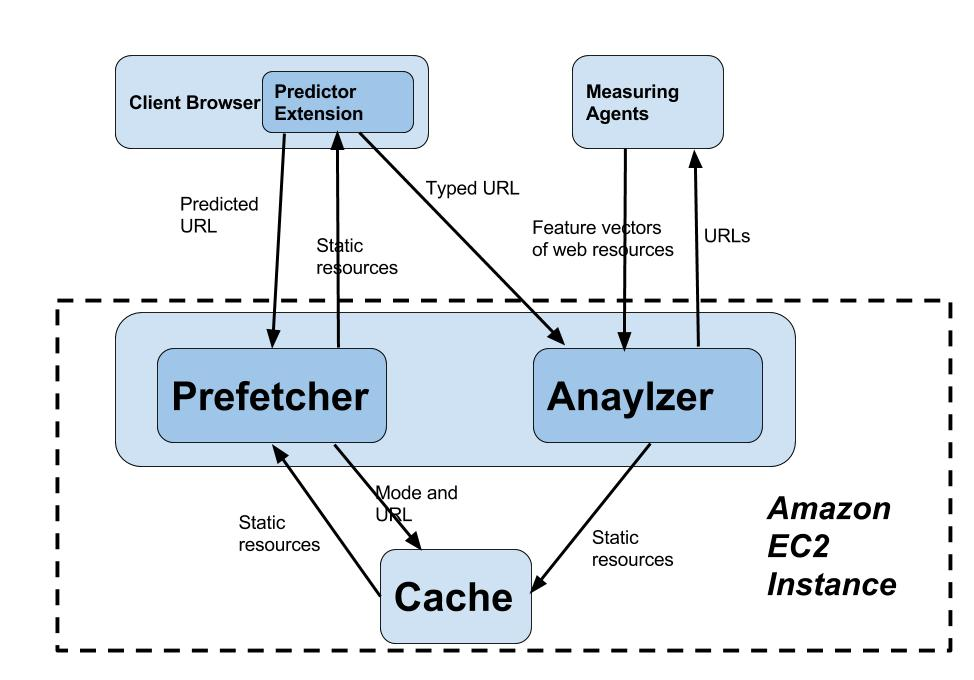
\includegraphics[width=0.5\textwidth]{ACCWeb-Arch-3.jpg}  
	\caption{AccWeb architecture.}
	\label{fig:arch}
\end{figure} 

\subsection{Analyzing}

Analyzer is a Python server running on Amazon EC2 instance. Analyzer gets all URLs the user has visited and then sends these URLs to Measuring Agents. Measuring Agents navigate these websites, record all feature vectors of web resources, and send them back to Analyzer. A feature vector includes the type of resources, the time of sending requests, the time of getting responses, and so on. After analyzing data (which will be explained in Section~\ref{sec:details}), Analyzer forms potential responses for prefetching, and stores them in the cache.

\subsection{Prediction}

Predictor is a Chrome extension running on client browser and is responsible for predicting. Predictor records the user's typed texts and navigated URLs, and builds a prediction table. Utilizing this table, we design an algorithm to predict the URL the user wants to navigate based on his/her current input in the address bar. Since Predictor stores all the data in the extension itself, when the user flushes the browsing history, it still can predict URL the user wants to navigate. Also, unlike Chrome, the set of URLs that will be prefetched in AccWeb is almost the same as the browsing history of the user, which allows much more flexibility. After Predictor sends the predicted URL to Prefetcher, Prefetcher will send back all resources that will be loaded. Details of our prediction algorithm will be explained in Section~\ref{sec:details}.

\subsection{Prefetching}

Prefetcher is a Python server running on Amazon EC2 instance. Depending on real-time network condition and the user's own preference, the user can select his/her favorite prefetching mode in the Chrome extension. The available modes are full mode, limit mode, image mode, script mode and DNS-prefetch mode. The details of these modes will be explained in Section~\ref{sec:details}. After receiving the predicted URL and the current mode from the extension, Prefetcher fetches corresponding resources from cache and sends them back to the extension.

As discussed, Chrome users currently have no choice to select which types of resources to preload. Since Chrome prefetches all static resources, the cost of misprediction is very high, especially if the network is on congestion. Using AccWeb, the user can choose the mode that meets his/her need as well as the network condition. On poor network condition, users may select limit mode or even DNS-prefetch mode to reduce the bandwidth of prefetching. Also, different users may have different preferences. The image mode and the script mode cater to these preferences.